\documentclass[aspectratio=169,11pt,t]{beamer}
% ============================================================
%  ksa-cs-v2: ksa-cs-lecture-template.tex 스타일 + 한글, v2 덱(16:9)용.
%    - 짙은 네이비 헤드라인 (섹션 이름 + 프레임마다 점)
%    - 꽉 찬 파란 제목 막대, 둥근 그림자 블록
%    - 한글: Noto Sans CJK KR (fontspec)
%  사용:
%    \documentclass[aspectratio=169,11pt,t]{beamer}
%    \input{<..>/theme/ksa-cs-v2.tex}
%  ksa-theme.tex 의 매크로(\kb \kq, ksablue/ksared 등)도 같은 이름으로 둔다
%  -> v2 덱 본문을 거의 그대로 옮길 수 있다.
% ============================================================

\usepackage{fontspec}
\usepackage{amsmath,amssymb}
\usepackage{tikz}
\usepackage{listings}
\usepackage{graphicx}
\usepackage{booktabs}
\usepackage{varwidth}
% enumitem 은 넣지 않는다 (beamer 글머리표가 사라진다)

\defaultfontfeatures{Ligatures=TeX}
\setmainfont{Noto Sans CJK KR}
\setsansfont{Noto Sans CJK KR}
\setmonofont{Noto Sans Mono CJK KR}[Scale=0.92]
\usefonttheme{professionalfonts}

% ---------- 기본 틀 ----------
\usetheme{default}
\useinnertheme[shadow=true]{rounded}
\setbeamertemplate{navigation symbols}{}
\setbeamersize{text margin left=1em,text margin right=1em}

% ---------- 색 (템플릿 원본 값) ----------
\definecolor{navydark}{HTML}{191959}
\definecolor{navydim}{HTML}{8888B0}
\definecolor{navytitle}{HTML}{262686}
\definecolor{navyblue}{HTML}{3333B2}
\definecolor{blockbodybg}{HTML}{E9E9F3}
\definecolor{examplegreen}{HTML}{006000}
\definecolor{examplebg}{HTML}{E5EFE5}
\definecolor{alertred}{HTML}{BF0000}
\definecolor{alertbg}{HTML}{F9E5E5}
% ksa-theme.tex 와 같은 이름 (본문 호환)
\colorlet{ksablue}{navytitle}
\colorlet{ksabluedk}{navydark}
\definecolor{ksagold}{HTML}{D6CBB1}
\definecolor{ksagolddk}{HTML}{A9976B}
\colorlet{ksared}{alertred}
\definecolor{ksagray}{HTML}{5B5B5B}

\setbeamercolor{structure}{fg=navyblue}
\setbeamercolor{alerted text}{fg=alertred}
\setbeamercolor{frametitle}{bg=navytitle,fg=white}
\setbeamercolor{title}{fg=white,bg=navytitle}
\setbeamercolor{block title}{bg=navytitle,fg=white}
\setbeamercolor{block body}{bg=blockbodybg,fg=black}
\setbeamercolor{block title example}{bg=examplegreen,fg=white}
\setbeamercolor{block body example}{bg=examplebg,fg=black}
\setbeamercolor{block title alerted}{bg=alertred,fg=white}
\setbeamercolor{block body alerted}{bg=alertbg,fg=black}
\setbeamercolor{item}{fg=navyblue}
\setbeamertemplate{itemize item}[circle]
\setbeamertemplate{itemize subitem}[triangle]

% ---------- 헤드라인: miniframes (섹션 이름 + 점) ----------
\useoutertheme[subsection=false]{miniframes}
\setbeamerfont{section in head/foot}{size=\tiny}
\setbeamercolor{section in head/foot}{bg=navydark,fg=white}
\setbeamercolor{mini frame}{fg=white}
\setbeamertemplate{mini frames}[circle]

% ---------- 제목 막대: 폭 꽉 채움, 두 줄까지 ----------
\setbeamerfont{frametitle}{size=\normalsize,series=\bfseries}
\setbeamertemplate{frametitle}{%
  \nointerlineskip
  \begin{beamercolorbox}[wd=\paperwidth,ht=2.7ex,dp=1.1ex,leftskip=.3cm,rightskip=.3cm]{frametitle}%
    \usebeamerfont{frametitle}\insertframetitle
  \end{beamercolorbox}}

% ---------- 쪽 번호: 오른쪽 아래 ----------
\setbeamertemplate{footline}{%
  \hfill
  {\color{navydim}\scriptsize\insertframenumber\,/\,\inserttotalframenumber}%
  \hspace{3mm}\vspace{2mm}%
}

% ---------- 표지: 템플릿처럼 헤드라인은 그대로, 가운데 둥근 그림자 상자에 제목 한 줄 ----------
% 덱에서:  {\setbeamertemplate{footline}{}\begin{frame}[c,noframenumbering]\titlepage\end{frame}}
\setbeamercolor{title}{fg=white,bg=navyblue}
\makeatletter
\setbeamertemplate{title page}{%
  \vfill
  \centering
  \begin{minipage}{0.84\paperwidth}
  \begin{beamercolorbox}[wd=\linewidth,sep=7pt,center,rounded=true,shadow=true]{title}
    {\usebeamerfont{title}\inserttitle\par}%
    \ifx\insertsubtitle\@empty\else\vskip0.4em{\usebeamerfont{subtitle}\insertsubtitle\par}\fi
  \end{beamercolorbox}
  \end{minipage}\par\vskip1.6em
  {\usebeamerfont{author}\color{navytitle}\insertauthor\par}\vskip0.3em
  {\usebeamerfont{institute}\color{ksagray}\insertinstitute\par}
  \vfill
}
\makeatother
\setbeamerfont{title}{series=\bfseries,size=\Large}
\setbeamerfont{subtitle}{size=\normalsize}
\setbeamerfont{author}{size=\normalsize}
\setbeamerfont{institute}{size=\small}

% ksa-theme 호환: 덱이 \renewcommand{\ksacredit}{..} 를 해도 되게 (꼬리말에는 안 쓴다)
\newcommand{\ksacredit}{}

% ---------- 강조 ----------
\newcommand{\hl}[1]{\textcolor{alertred}{#1}}
\newcommand{\hlb}[1]{\textcolor{navyblue}{#1}}
\newcommand{\kb}[1]{\textbf{\color{ksablue}#1}}
\newcommand{\kq}[1]{\textbf{\color{ksared}#1}}

% ---------- 파이썬 코드 (템플릿과 같은 색) ----------
\definecolor{codekw}{HTML}{0033B3}
\definecolor{codebuiltin}{HTML}{BF0000}
\definecolor{codestr}{HTML}{067D17}
\definecolor{codecomment}{HTML}{8C8C8C}
\definecolor{codenum}{HTML}{1750EB}
\lstdefinestyle{py}{
  language=Python, basicstyle=\ttfamily\scriptsize,
  keywordstyle=\color{codekw}\bfseries, stringstyle=\color{codestr},
  commentstyle=\color{codecomment}\itshape, numberstyle=\color{codenum},
  emph={print,len,range,sum,input,int,str,float,list,dict,append,remove,sorted,abs,min,max},
  emphstyle=\color{codebuiltin}, showstringspaces=false, keepspaces=true,
  columns=fixed, basewidth=0.52em, aboveskip=1mm, belowskip=1mm, xleftmargin=2mm,
  breaklines=true
}
\lstset{style=py}

% 원본 덱 (ksa-theme): slides/v2/ml1/week14/bert/ -- 그림은 거기 figs/ 를 그대로 쓴다
\setbeamerfont{author}{size=\normalsize}
\setbeamerfont{institute}{size=\small}
\graphicspath{{../../../v2/ml1/week14/bert/figs/}{../../../assets/}}
\makeatletter
\newcommand{\markpage}[1]{\protected@write\@auxout{}{\string\newlabel{#1}{{\the\c@framenumber}{}}}\hypertarget{#1}{}}
\newcommand{\pref}[1]{\hyperlink{#1}{\textcolor{ksagolddk}{(p.\ref{#1})}}}
\makeatother

\renewcommand{\ksacredit}{Machine Learning and Deep Learning \,\textperiodcentered\, BERT}
\title{BERT 빈칸 채우기}
\subtitle{빈칸의 앞뒤를 모두 보고 배운다}
\author{Machine Learning and Deep Learning}
\institute{한국과학영재학교 (KSA)}
\date{}
\begin{document}
{\setbeamertemplate{footline}{}\begin{frame}[c,noframenumbering]\titlepage\end{frame}}


\section{질문}
% --- 오늘의 질문
\begin{frame}{오늘의 질문: 앞부분이 같으면 빈칸도 같을까?}
\vfill
\centering
{\LARGE I went to the \kb{\_\_\_\_} to buy some bread.}\\[0.5em]
{\LARGE I went to the \kq{\_\_\_\_} to see a doctor.}\vskip0.8em
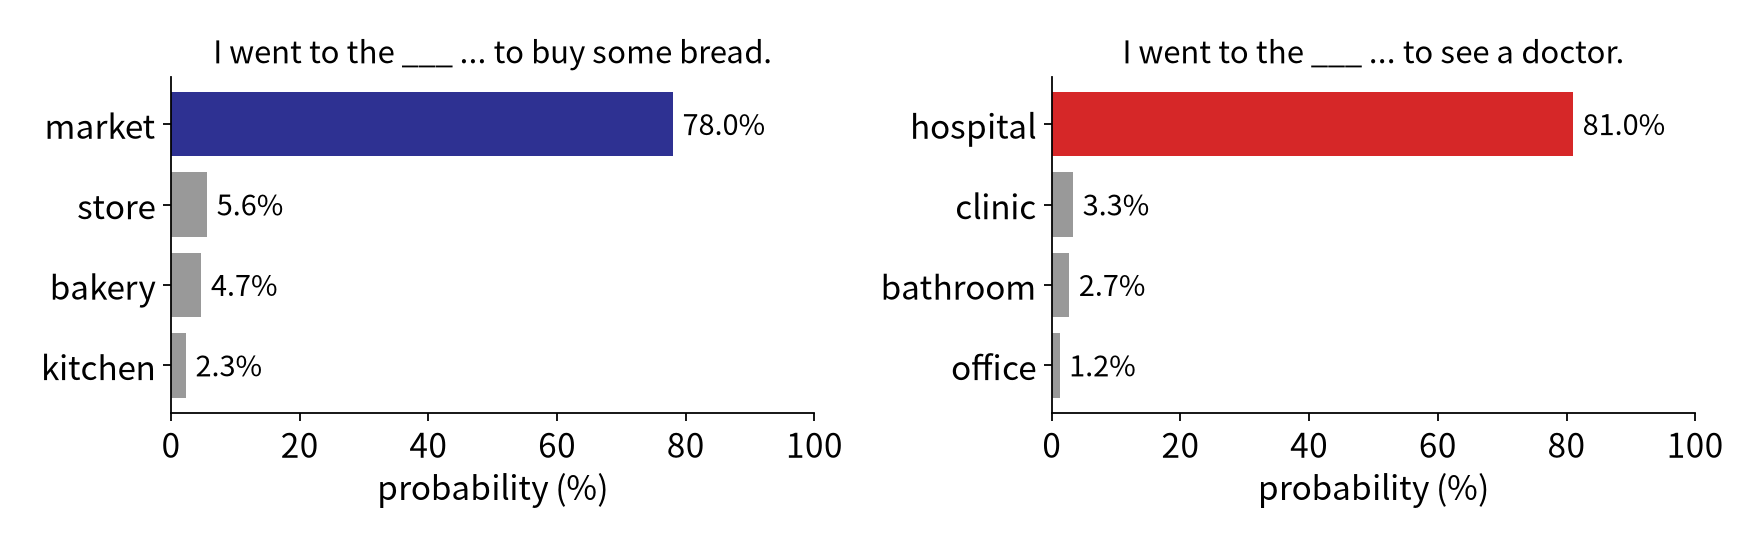
\includegraphics[width=0.8\linewidth]{bert_fill.png}\par
{\large 실제 BERT 가 고른 단어 \quad 빈칸 \textbf{뒤}를 보고 답을 바꾼다}
\vfill
\note{두 문장의 앞부분은 똑같이 I went to the입니다. 빈칸에 들어갈 말도 같을까요? 실제 BERT에 넣어 보면, 빵을 사러 갔다면 market을 78퍼센트, 의사를 만나러 갔다면 hospital을 81퍼센트로 고릅니다. 빈칸 뒤에 나오는 단어를 보고 답을 바꾼 겁니다. 앞만 보고 다음 단어를 맞히는 GPT로는 이 빈칸을 이렇게 채울 수 없습니다. 오늘은 앞뒤를 모두 보는 BERT를 배웁니다.}
\end{frame}

\section{BERT}
% --- BERT 란
\begin{frame}{BERT: 양방향 트랜스포머 인코더}
\vfill
\centering
{\large \textbf{B}idirectional \textbf{E}ncoder \textbf{R}epresentations from \textbf{T}ransformers}\\[0.1em]{\normalsize Devlin 외 (Google, 2018)}\vskip0.4em
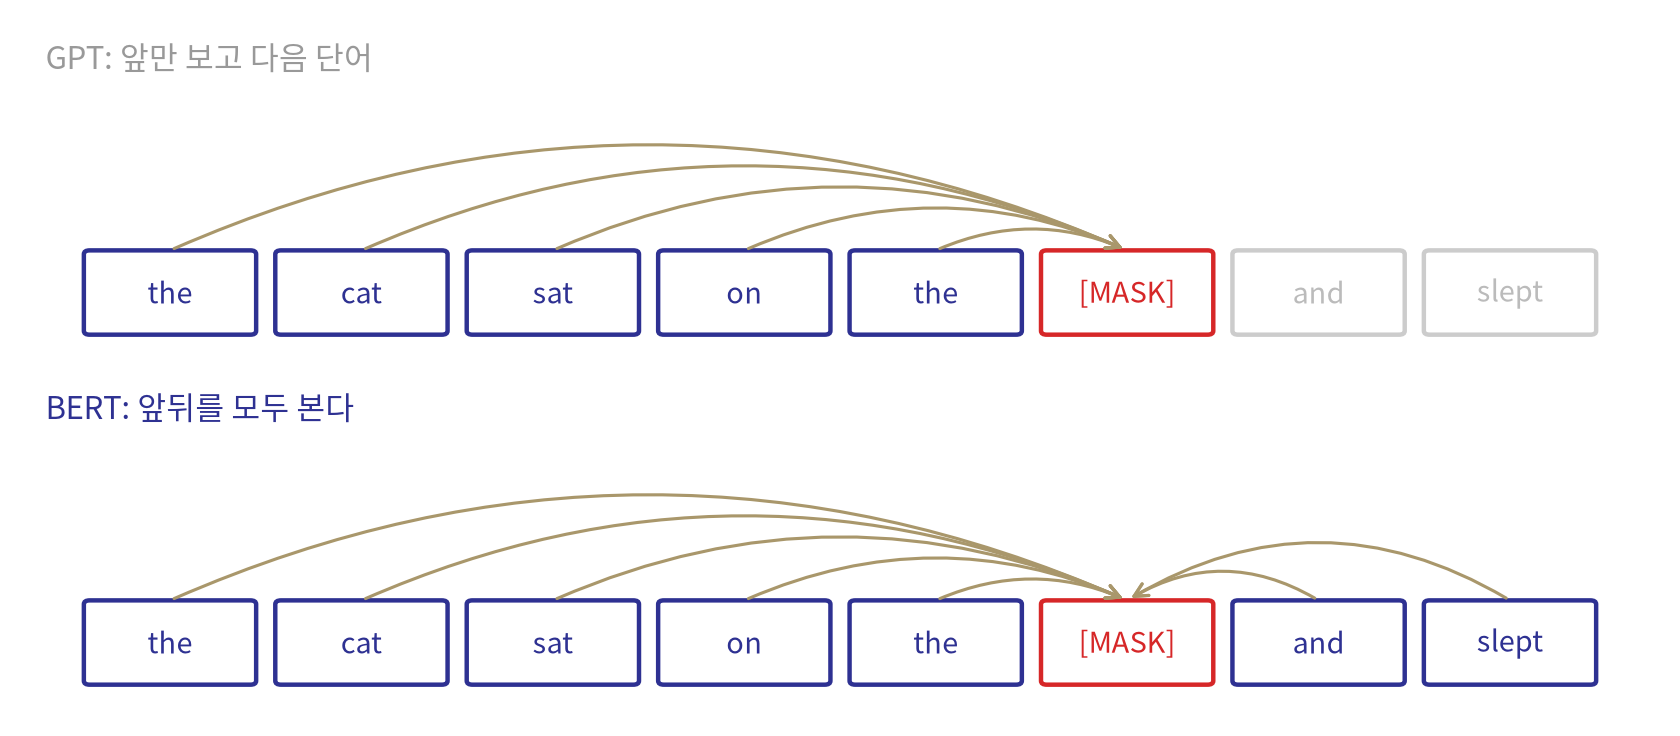
\includegraphics[width=0.70\linewidth]{bert_dir.png}\par
{\large 12주차 트랜스포머에서 \textbf{인코더만}: 마스크 없이 모든 단어가 모든 단어를 본다}
\vfill
\note{BERT는 Bidirectional Encoder Representations from Transformers의 줄임말로, 2018년 구글의 데블린 팀이 발표했습니다. 12주차에 트랜스포머를 배울 때, GPT는 디코더만 써서 앞만 보는 마스크를 씌웠고, BERT는 인코더만 쓴다고 했습니다. 마스크가 없으니 모든 단어가 모든 단어를 봅니다. 그래서 빈칸을 채울 때 앞의 the cat sat on the뿐 아니라 뒤의 and slept까지 봅니다.}
\end{frame}

% --- 학습법
\begin{frame}{학습: 빈칸 채우기 (Masked Language Model)}
\markpage{mlm}
\vfill
\centering
{\large 문장 속 토큰의 \kb{15\%} 를 골라 맞히게 한다}\vskip0.4em
\renewcommand{\arraystretch}{1.5}
{\large\begin{tabular}{lll}
고른 토큰의 80\% & \texttt{[MASK]} 로 바꾼다 & the cat sat on the \texttt{[MASK]}\\
10\% & 아무 단어로 바꾼다 & the cat sat on the \textit{apple}\\
10\% & 그대로 둔다 & the cat sat on the \textit{mat}
\end{tabular}}\vskip0.6em
{\large 왜 섞나: 실제로 쓸 때는 \texttt{[MASK]} 가 없으니까}\\[0.4em]
{\large 책 8억 + 위키백과 25억 단어 \quad 이름표 없이 (\textbf{자기 지도 학습})}
\vfill
\note{BERT의 학습법은 빈칸 채우기입니다. 문장 속 토큰의 15퍼센트를 골라 원래 단어를 맞히게 합니다. 고른 토큰의 80퍼센트는 MASK로 바꾸고, 10퍼센트는 아무 단어로, 10퍼센트는 그대로 둡니다. 왜 이렇게 섞을까요? 실제로 쓸 때는 MASK가 없으니, MASK 자리만이 아니라 모든 단어의 벡터를 잘 만들어야 하기 때문입니다. 데이터는 책 8억 단어와 위키백과 25억 단어인데, 정답이 원래 문장에 들어 있어 사람이 이름표를 달 필요가 없습니다. 이런 방식을 자기 지도 학습이라 합니다. 원 논문은 두 문장이 이어지는지 맞히는 과제도 함께 썼습니다.}
\end{frame}

% --- 크기
\begin{frame}{손으로 세기: BERT-base 의 가중치}
\vfill
\centering
\renewcommand{\arraystretch}{1.5}
{\large\begin{tabular}{lll}
단어 표 & 30,522 단어 × 768칸 & 2,344만\\
블록 하나 & $\approx 12 d^2 = 12 \times 768^2$ (12주차) & 708만\\
블록 12개 & & 8,505만\\\hline
합 (위치 · 정규화 포함) & & \kb{1억 889만} $\approx$ 110M
\end{tabular}}\vskip0.8em
{\large BERT-large: 24층 · 1,024칸 $\to$ 340M \quad 머리 수: base 12, large 16}\\[0.2em]
{\small 실제 Hugging Face \texttt{bert-base-uncased} 로 센 값}
\vfill
\note{BERT-base의 가중치를 세어 봅시다. 단어 표가 30522개 단어 곱하기 768칸, 약 2344만 개입니다. 12주차에 배운 대로 트랜스포머 블록 하나는 약 12 d 제곱, 12 곱하기 768 제곱, 약 708만 개이고, 12층이면 8505만 개입니다. 위치 벡터와 정규화까지 더하면 1억 889만 개, 논문의 110M입니다. 실제 모델로 센 값과 맞습니다. BERT-large는 24층에 1024칸, 340M입니다.}
\end{frame}

\section{실험}
% --- 실험 빈칸
\begin{frame}{실험: 실제 BERT 에 빈칸 넣기}
\markpage{fill}
\vfill
\centering
\renewcommand{\arraystretch}{1.4}
{\normalsize\begin{tabular}{lll}
문장 & 1위 & 2 · 3위 (\%)\\\hline
I went to the \_\_\_ to buy some bread. & market \kb{78.0\%} & store 5.6, bakery 4.7\\
I went to the \_\_\_ to see a doctor. & hospital \kb{81.0\%} & clinic 3.3\\
The capital of France is \_\_\_. & paris \kb{41.7\%} & lille 7.1, lyon 6.3\\
The capital of Korea is \_\_\_. & seoul \kb{99.8\%} &
\end{tabular}}\vskip0.6em
{\large 문법 (어떤 품사가 와야 하나) 과 지식 (수도) 을 함께 배웠다}\\[0.2em]
{\small \texttt{bert-base-uncased}, 소문자만 쓰는 모델}
\vfill
\note{실제 BERT에 빈칸 문장을 넣어 봤습니다. 빵이면 market 78퍼센트, 의사면 hospital 81퍼센트입니다. 프랑스의 수도는 paris를 41.7퍼센트로 1위로 골랐고, lille과 lyon 같은 프랑스 도시가 뒤를 잇습니다. 한국의 수도는 seoul을 99.8퍼센트로 골랐습니다. 빈칸 채우기만 했는데 어떤 품사가 와야 하는지 같은 문법과, 수도 같은 세상 지식을 함께 배운 겁니다.}
\end{frame}

% --- 문맥 벡터
\begin{frame}{같은 단어, 문맥마다 다른 벡터}
\markpage{bank}
\vfill
\begin{columns}[c]
\column{0.55\linewidth}\centering
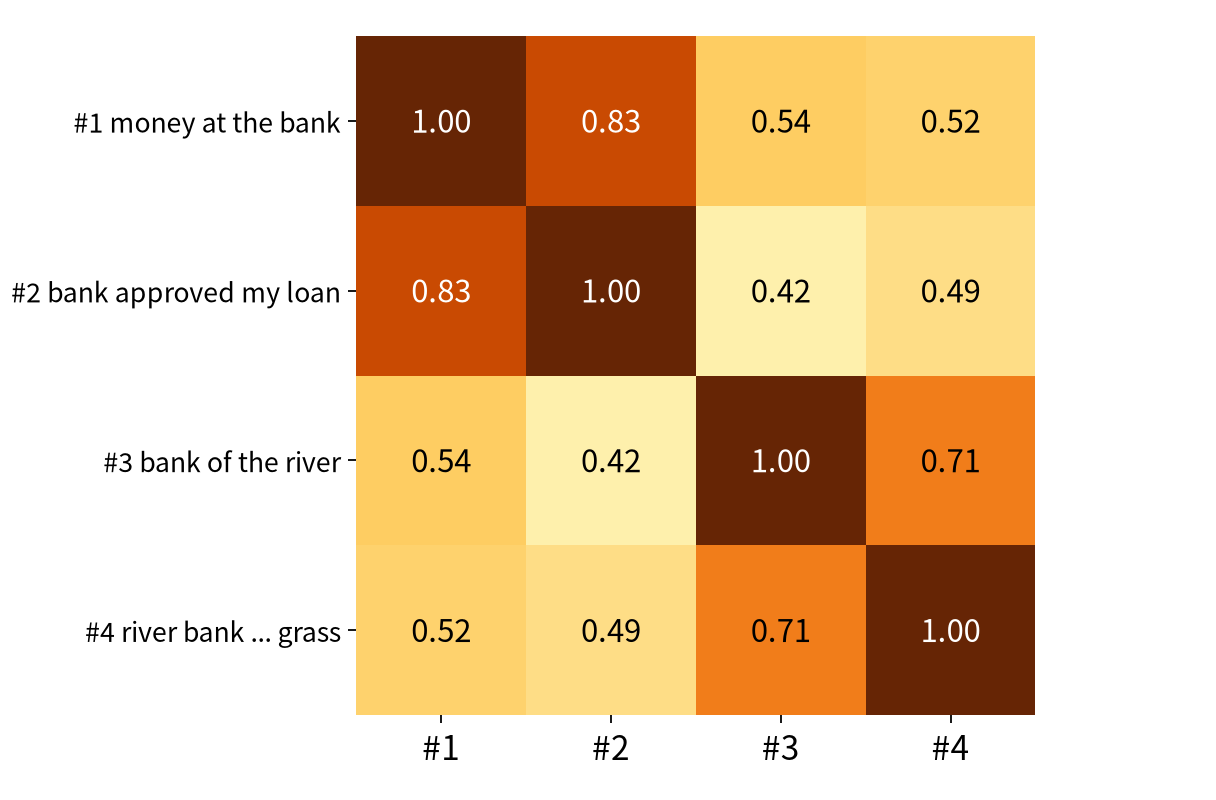
\includegraphics[width=\linewidth]{bert_bank.png}
\column{0.43\linewidth}
{\large ``bank'' 의 마지막 층 벡터, 코사인 유사도}\\[0.6em]
{\large 은행끼리 \kb{0.83}, 강둑끼리 \kb{0.71}}\\[0.2em]
{\large 은행 $\leftrightarrow$ 강둑 \kq{0.42 $\sim$ 0.54}}\\[0.8em]
{\large word2vec: ``bank'' 는 벡터 \textbf{하나}}\\
{\large BERT: 문장마다 다른 벡터}\\[0.3em]
{\small 문맥을 담은 임베딩 (contextual embedding)}
\end{columns}
\vfill
\note{BERT의 또 다른 힘은 같은 단어라도 문맥마다 다른 벡터를 준다는 겁니다. bank가 들어간 문장 넷, 은행 뜻 둘과 강둑 뜻 둘에서 bank 자리의 마지막 층 벡터를 꺼내 코사인 유사도를 쟀습니다. 은행끼리는 0.83, 강둑끼리는 0.71이고, 은행과 강둑 사이는 0.42에서 0.54입니다. word2vec에서는 bank가 벡터 하나뿐이라 두 뜻이 섞였는데, BERT는 문장을 보고 뜻을 가려냅니다. 이런 걸 문맥을 담은 임베딩이라고 합니다.}
\end{frame}

\section{미세조정}
% --- 사전학습 + 미세조정
\begin{frame}{사전학습 + 미세조정}
\vfill
\centering
\renewcommand{\arraystretch}{1.5}
{\large\begin{tabular}{lll}
1단계 \textbf{사전학습} & 빈칸 채우기, 33억 단어 & 비싸지만 한 번만\\
2단계 \textbf{미세조정} & 과제의 이름표 데이터 & \texttt{[CLS]} 벡터 + 분류기, 몇 바퀴
\end{tabular}}\vskip0.8em
{\large 언어 과제 \kb{11}개 최고 기록 \quad GLUE \kb{80.5\%} (+7.7\%p)}\\[0.3em]
{\large 감정 분류 · 문장 관계 · 질문 답 찾기를 BERT 하나로}\\[0.2em]
{\small 9주차 전이 학습 (ImageNet 사전학습 CNN) 과 같은 생각}
\vfill
\note{BERT는 두 단계로 씁니다. 먼저 빈칸 채우기로 33억 단어를 학습하는 사전학습을 한 번 합니다. 비싸지만 한 번이면 됩니다. 그다음 풀고 싶은 과제의 이름표 데이터로 미세조정을 합니다. 맨 앞에 붙는 CLS 토큰의 벡터에 분류기를 하나 얹어 몇 바퀴만 더 학습합니다. 이렇게 해서 언어 과제 11개에서 최고 기록을 냈고, 여러 과제의 평균인 GLUE 점수는 80.5퍼센트로 이전보다 7.7퍼센트포인트 높았습니다. 9주차에 ImageNet으로 미리 학습한 CNN을 가져다 쓰던 전이 학습과 같은 생각입니다.}
\end{frame}

% --- 편향
\begin{frame}{배운 글의 편향도 배운다}
\vfill
\centering
\renewcommand{\arraystretch}{1.4}
{\large\begin{tabular}{lll}
문장 & 1위 & 다른 후보\\\hline
\textbf{She} is a \_\_\_ at the hospital. & nurse \kq{60.9\%} & patient 11.0, doctor 10.9\\
\textbf{He} is a \_\_\_ at the hospital. & doctor \kq{28.7\%} & patient 22.5, nurse 17.5
\end{tabular}}\vskip0.8em
{\large 대명사 하나만 바꿨는데 직업이 바뀐다: 글 속 고정관념이 확률에}\\[0.3em]
{\large 채용 · 추천에 쓰면 편향이 결정이 된다 $\to$ 편향을 재고 점검해야}
\vfill
\note{조심할 점도 있습니다. She is a 빈칸 at the hospital에서는 nurse를 60.9퍼센트, He is a 빈칸 at the hospital에서는 doctor를 28.7퍼센트로 골랐습니다. 대명사 하나만 바꿨는데 직업이 바뀝니다. 학습한 책과 위키백과에 있는 고정관념이 확률에 그대로 들어간 겁니다. 이런 모델을 채용이나 추천에 그대로 쓰면 편향이 결정이 됩니다. 그래서 데이터를 점검하고 편향을 재는 일이 함께 필요합니다.}
\end{frame}

% --- 이후
\begin{frame}{BERT 이후}
\vfill
\centering
\renewcommand{\arraystretch}{1.5}
{\large\begin{tabular}{ll}
2019 & 구글 검색에 BERT 적용 (영어 검색어 10곳 중 1곳)\\
2019 & RoBERTa (더 오래 · 더 많이), ALBERT, DistilBERT (작게)\\
2019 & Sentence-BERT: 문장 임베딩 $\to$ 의미 검색, RAG\\
2020 $\sim$ & 생성은 GPT 계열로: 글을 \textbf{쓰는} 일은 앞만 보는 모델이 맡았다
\end{tabular}}\vskip0.8em
{\large BERT: 글을 \textbf{이해}하는 일 (검색 · 분류) \quad GPT: 글을 \textbf{쓰는} 일}
\vfill
\note{BERT는 2019년 구글 검색에 들어가 영어 검색어 10개 중 1개를 더 잘 이해하게 됐다고 발표됐습니다. 같은 해 더 오래, 더 많이 학습한 RoBERTa, 작게 만든 ALBERT와 DistilBERT가 나왔고, 문장 임베딩을 만드는 Sentence-BERT는 지난 덱에서 본 의미 검색과 RAG의 바탕이 됐습니다. 반면 글을 쓰는 일은 앞만 보는 GPT 계열이 맡게 됐습니다. 정리하면 BERT는 글을 이해하는 일, GPT는 글을 쓰는 일에 강합니다.}
\end{frame}

\section{연습}
% --- 문제풀이
\begin{frame}{문제풀이}
\vfill
\begin{enumerate}
\item 토큰 200개 문장에서 몇 개를 골라 맞히게 하나? 그중 \texttt{[MASK]} 로 바뀌는 것은 대략 몇 개?\vskip0.8em
\item BERT-large (24층, $d = 1024$) 의 블록 가중치를 $12 d^2$ 로 어림하면?\vskip0.8em
\item GPT 로 ``I went to the \_\_\_ to see a doctor.'' 의 빈칸을 채우기 어려운 이유는?\vskip0.8em
\item word2vec 으로 bank 의 두 문장 유사도를 재면 얼마가 나올까?
\end{enumerate}
\vfill
\note{1번 답. 15퍼센트, 30개를 고르고, 그중 80퍼센트, 24개가 MASK로 바뀝니다. 2번 답. 12 곱하기 1024 제곱 곱하기 24, 약 3억 200만 개입니다. 단어 표를 더하면 340M에 가깝습니다. 3번 답. GPT는 빈칸 앞의 I went to the만 보고 다음 단어를 고르니, 뒤에 나오는 see a doctor를 쓸 수 없습니다. 4번 답. word2vec은 bank에 벡터가 하나뿐이니 어느 문장이든 같은 벡터, 유사도 1입니다.}
\end{frame}

% --- 실습
\begin{frame}{실습}
\vfill
\centering\begin{tabular}{rl}
\large 1 & 15\% 가리기 (80 / 10 / 10) 직접 구현\\[0.5em]
\large 2 & 실제 BERT 로 빈칸 채우기, 내 문장 넣어 보기\\[0.5em]
\large 3 & 문맥 벡터: ``bank'' 유사도, 가중치 수 세기
\end{tabular}\vskip1em
Hugging Face \texttt{bert-base-uncased} \\[0.4em]\href{https://colab.research.google.com/github/SuminHan/book-ml/blob/main/slides/v2/ml1/week14/bert/lab/bert.ipynb}{\textcolor{ksagolddk}{▶ Colab에서 실습 노트북 열기}}
\vfill
\note{실습은 세 부분입니다. 첫째, 15퍼센트를 골라 80, 10, 10으로 가리는 과정을 직접 구현합니다. 둘째, 실제 BERT로 빈칸을 채우고 여러분의 문장도 넣어 봅니다. 셋째, bank의 문맥 벡터 유사도를 재고 가중치 수를 세어 봅니다.}
\end{frame}

\section{정리}
% --- 정리
\begin{frame}{정리}
\vfill
\centering\large\begin{tabular}{l}
\textbf{BERT}: 트랜스포머 \textbf{인코더}, 빈칸의 \kb{앞뒤}를 모두 본다 (2018)\\[0.5em]
학습: 토큰 15\% 빈칸 채우기 (80 / 10 / 10), 이름표 없이 33억 단어\\[0.5em]
bread $\to$ market 78\%, doctor $\to$ hospital 81\% \quad bank: 뜻마다 다른 벡터\\[0.5em]
사전학습 + 미세조정: 11개 과제 최고 \quad 편향도 배운다 (she $\to$ nurse 61\%)
\end{tabular}
\vfill
\note{정리합니다. BERT는 트랜스포머의 인코더만 써서 빈칸의 앞뒤를 모두 봅니다. 토큰 15퍼센트를 가리고 맞히는 빈칸 채우기로, 이름표 없이 33억 단어를 학습했습니다. 빵이면 market, 의사면 hospital을 고르고, bank는 뜻마다 다른 벡터를 줍니다. 사전학습한 BERT를 조금씩 미세조정해 11개 과제에서 최고 기록을 냈지만, 글에 있는 편향도 함께 배웁니다.}
\end{frame}
\end{document}
